\documentclass[twocolumn]{article}

% --- Idioma y codificación ---
\usepackage[utf8]{inputenc}
\usepackage[T1]{fontenc}

% --- Matemáticas ---
\usepackage{amsmath, amssymb}

% --- Microtipografía (IMPORTANTE: sin expansión para evitar error de pdfTeX) ---
\usepackage[protrusion=true,expansion=false]{microtype}

% --- Gráficas y captions ---
\usepackage{graphicx}
\usepackage{caption}

% --- Links / rutas ---
\usepackage[hidelinks]{hyperref}

% --- Listas compactas ---
\usepackage{enumitem}
\setlist[itemize]{noitemsep, topsep=2pt, leftmargin=*}

\title{\textbf{Optimización del problema ``Subir Escaleras''}:\\
de recursión exponencial a fórmula cerrada (Binet)}
\author{\textbf{Participantes:} Jhon Perlaza, Heidi Sofía Barrera, Andrés Felipe Cadena, Juan Ahumada}
\date{29 de mayo de 2026}

\begin{document}
\maketitle

\begin{abstract}
Este trabajo estudia el problema clásico de contar cuántas formas existen de subir $n$ escalones utilizando pasos de tamaño 1 o 2. Se implementa una solución recursiva ingenua sin memoización, cuyo tiempo crece exponencialmente, y se compara contra una implementación optimizada basada en la relación con Fibonacci y la fórmula cerrada de Binet. Se presenta un análisis de complejidad y un benchmarking que evidencia la diferencia de escalabilidad a medida que $n$ aumenta.
\end{abstract}

\section{Introducción}
Definimos $W(n)$ como el número de formas de subir $n$ escalones cuando se permiten saltos de 1 o 2. Cada forma termina con un paso de 1 desde $n-1$ o un paso de 2 desde $n-2$, por lo que se cumple:
\begin{equation}
W(n) = W(n-1) + W(n-2), \quad W(0)=1,\; W(1)=1.
\end{equation}
Esta recurrencia conecta el problema con Fibonacci y permite obtener mejoras drásticas en complejidad temporal.

\section{Desarrollo matemático}
Sea $F(n)$ la sucesión de Fibonacci con $F(0)=0$ y $F(1)=1$. Se verifica (por inducción) que:
\begin{equation}
W(n)=F(n+1).
\end{equation}

\subsection{Implementación pesada: recursión ingenua}
La implementación pesada calcula $W(n)$ aplicando recursión directa sin guardar resultados intermedios. Si $T(n)$ representa el tiempo (número de llamadas), entonces:
\begin{equation}
T(n)=T(n-1)+T(n-2)+O(1).
\end{equation}
Esta recurrencia crece exponencialmente y se tiene:
\begin{equation}
T(n)=\Theta(\varphi^n),
\end{equation}
donde $\varphi=\frac{1+\sqrt{5}}{2}\approx 1.618$ es la proporción áurea. Por tanto, \textbf{no} es $O(n^2)$: el árbol de recursión se expande de forma explosiva.

\subsection{Implementación optimizada: fórmula cerrada (Binet)}
Usando la fórmula de Binet:
\begin{equation}
F(k)=\frac{\varphi^k-\psi^k}{\sqrt{5}},
\quad
\psi=\frac{1-\sqrt{5}}{2},
\end{equation}
y como $W(n)=F(n+1)$, puede calcularse el resultado mediante una expresión cerrada.

\textbf{Discusión de complejidad.} En un modelo ideal (evaluar una fórmula sin iterar hasta $n$), esta aproximación puede describirse como $O(1)$ en pasos matemáticos. En una implementación exacta, el costo real depende del tamaño del número (cantidad de dígitos) para $n$ grande. Aun así, la mejora frente a $\Theta(\varphi^n)$ es enorme y se evidencia empíricamente.

\section{Resultados experimentales (Benchmark)}
Se implementó un script de benchmarking en Python que compara:
\begin{itemize}
\item \textbf{Pesada (exponencial):} recursión ingenua sin memoización.
\item \textbf{Optimizada (``O(1)''):} Binet híbrida (usa \texttt{float} para $n$ pequeño y \texttt{decimal} para $n$ grande).
\end{itemize}

Para evitar tiempos excesivos, la versión exponencial se omite para $n>35$. El benchmark genera los archivos en la carpeta \path{results/}:
\begin{itemize}
\item \path{benchmark.csv}
\item \path{benchmark.png} (escala log--log)
\item \path{benchmark_small.png} (zoom para $n \le 35$)
\end{itemize}

\begin{figure}[h]
\centering
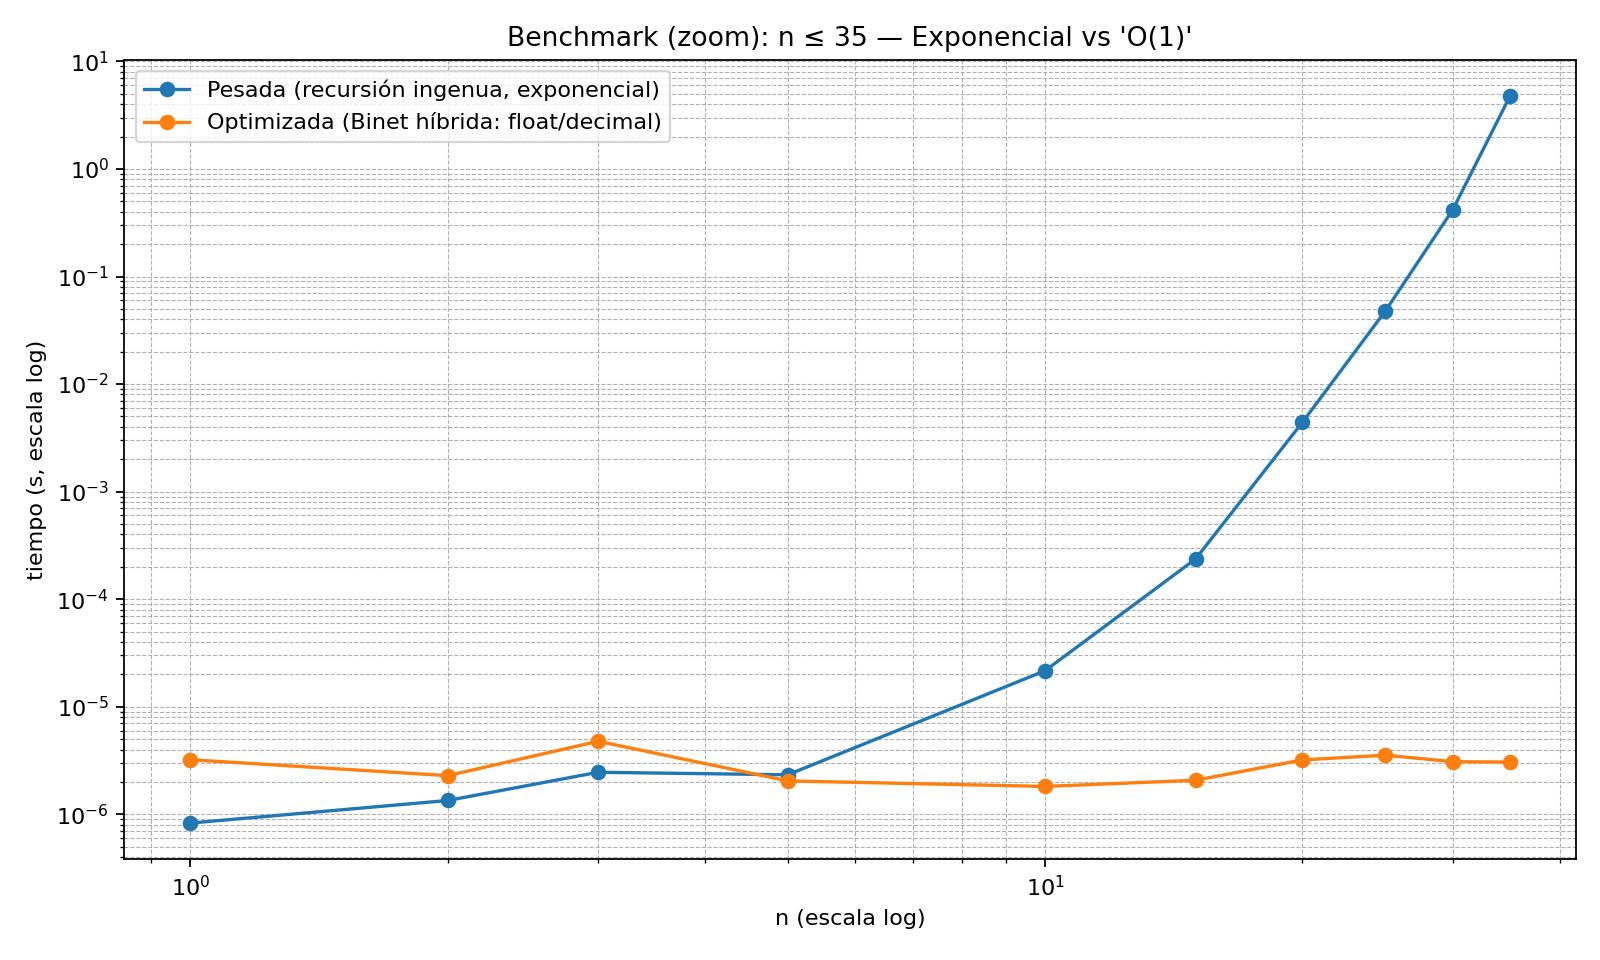
\includegraphics[width=\linewidth]{results/benchmark_small.png}
\caption{Comparación en escala log--log para $n\le 35$ (ambos algoritmos medidos).}
\end{figure}

\begin{figure}[h]
\centering
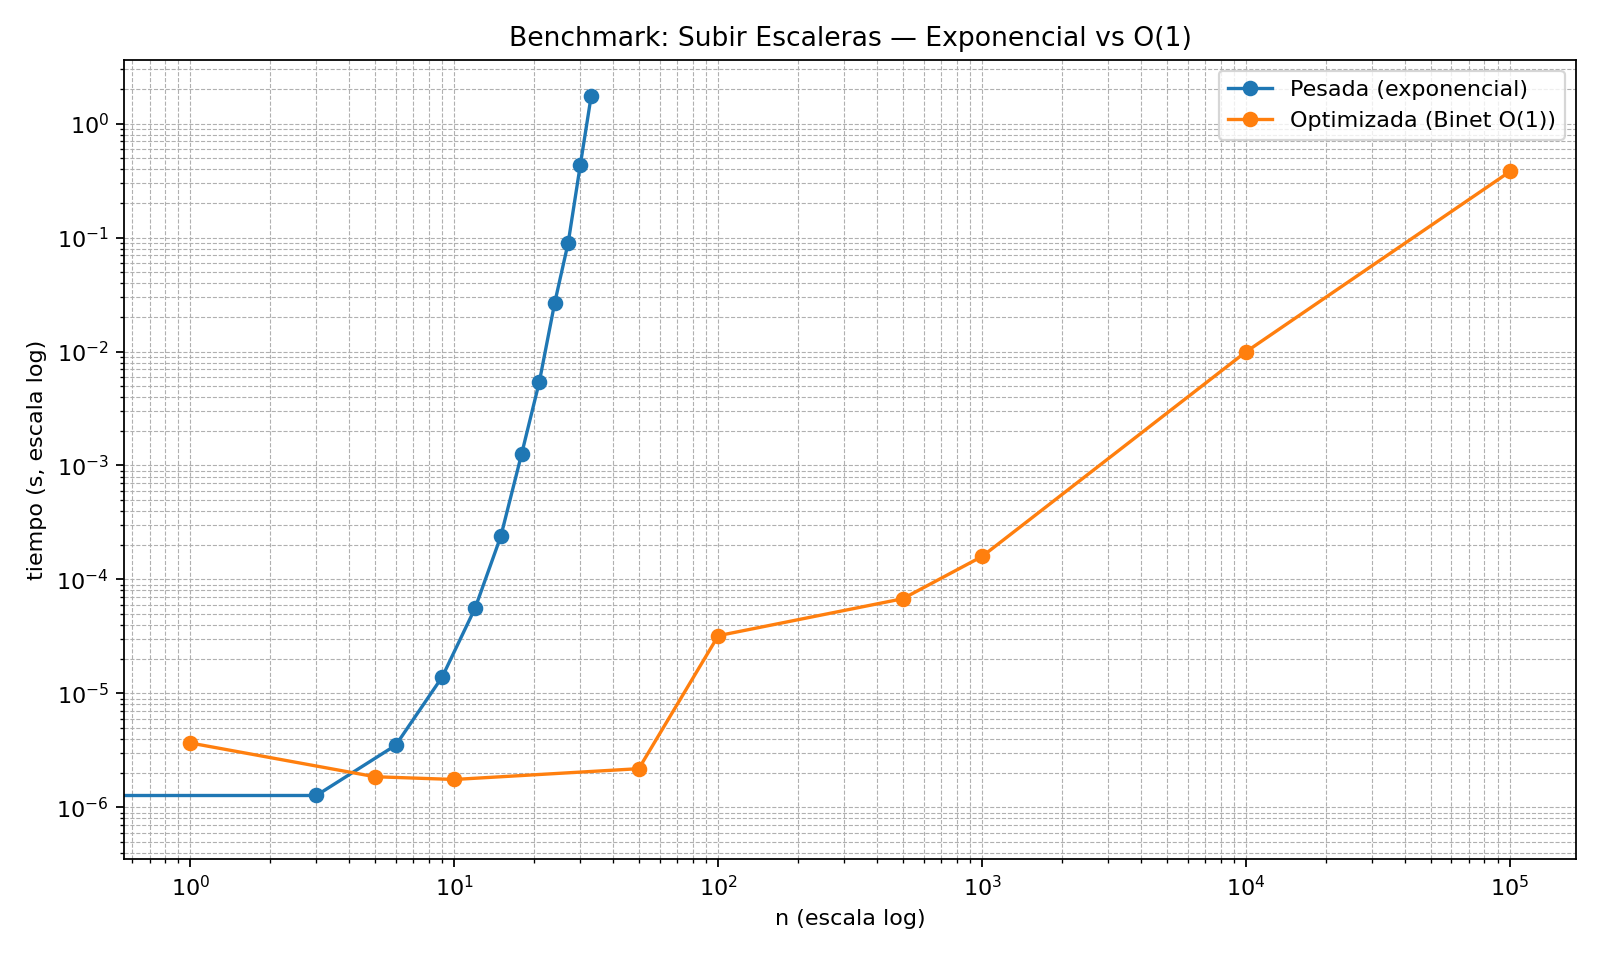
\includegraphics[width=\linewidth]{results/benchmark.png}
\caption{Comparación log--log para la lista completa. El exponencial aparece solo hasta $n=35$ (luego se omite).}
\end{figure}

\section{Aplicaciones reales}
La reducción de complejidad mediante matemáticas, precomputación o estructuras eficientes aparece en:
\begin{itemize}
\item \textbf{Bases de datos:} índices (B-trees, hashing) aceleran búsquedas de escaneo lineal a $O(\log n)$ u $O(1)$ promedio.
\item \textbf{Criptografía:} técnicas como exponenciación rápida reducen costos de $O(n)$ a $O(\log n)$.
\item \textbf{Programación dinámica:} memoización transforma recursiones exponenciales en soluciones polinómicas.
\end{itemize}

\section{Repositorio}
Código fuente ():\\
\url{https://github.com/JhonPerlaza0614/Entrega-Final.git}

\section{Referencias}
\begin{itemize}
\item E. W. Weisstein, ``Fibonacci Number'', \emph{MathWorld}. \url{https://mathworld.wolfram.com/FibonacciNumber.html}
\item Wikipedia, ``Fibonacci number'' y ``Binet's formula''. \url{https://en.wikipedia.org/wiki/Fibonacci_number}
\end{itemize}

\end{document}